%%%%%%%%%% CAPITOLO DI TESI %%%%%%%%%%
%
% Capitolo "3" Capitolo 3
%
%%%%%%%%%%%%%%%%%%%%%%%%%%%%%%%%%%%%%%
\mcchap{Progettazione}{cap:cap3}
\section{Entità ed associazioni}
Nella fase di progettazione concettuale del tool, uno dei principali
obiettivi è stata la definizione di un modello di dati che potesse 
supportare le funzionalità principali dell'applicazione.
A tal fine, si è deciso di realizzare un database relazionale che 
contenesse diverse tabelle. La creazione delle tabelle è gestita 
tramite Django, un framework Python molto conosciuto nello sviluppo di 
applicativi backend, verrà dettagliato in seguito.\\

Il database relazionale comprende quindi diverse tabelle, tra cui:
\begin{itemize}
\item campaign: la tabella principale del database, che rappresenta una 
campagna di aggiornamento. Ogni record in questa tabella contiene 
informazioni sulle specifiche della campagna;
\item item: tabella che contiene l'insieme dei server che devono essere 
aggiornati, correlati alla campagna tramite una relazione uno-a-molti. 
Ogni record in questa tabella rappresenta un singolo server da aggiornare;
\item updatefile: tabella che rappresenta i file di aggiornamento 
effettivi che verranno installati sui server selezionati. 
Anche questa tabella è correlata alla tabella "campaign" tramite una 
relazione uno-a-molti e contiene un record per ogni diverso sistema 
operativo dei server selezionati in una campagna di aggiornamento;
\item updatejob: tabella che contiene le informazioni sulle sessioni 
di aggiornamento avviate su un server. Ogni record in questa tabella 
rappresenta un'operazione di aggiornamento. È possibile avere più operazioni 
di aggiornamento per un singolo server, per consentire di ripetere 
l’aggiornamento in caso di fallimento;
\item updatejobstatushistory: tabella che tiene traccia dello stato di 
avanzamento dell’operazione di aggiornamento. Questa tabella è utilizzata 
per tenere traccia degli stati di ogni singola operazione di aggiornamento 
presente nella tabella.
\end{itemize}

\begin{figure}[H]
  \begin{flushright}
    \centering
    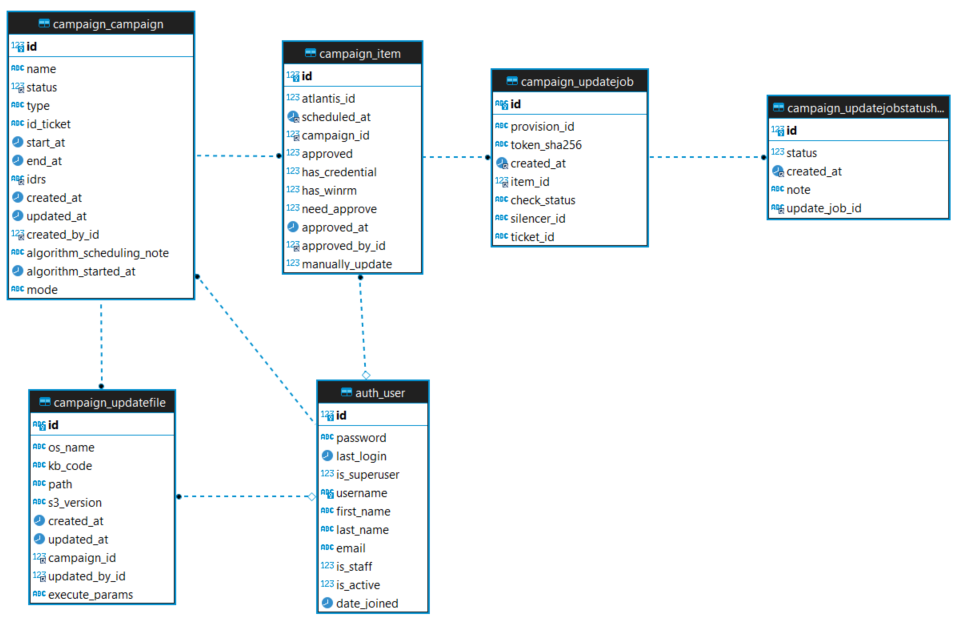
\includegraphics[width=0.90\textwidth]{imgs/ER_schema.png}
    \caption{Schema entità-relazione database relazionale}
    \label{fig:Schema entità-relazione database relazionale}
  \end{flushright}
\end{figure}

Come mostra l’immagine dello schema ER, le tabelle del database sono state 
progettate in modo da riflettere le relazioni tra le entità coinvolte 
nel sistema.

La tabella "item" è correlata alla tabella "campaign" attraverso una 
relazione uno-a-molti, in quanto ad ogni campagna di aggiornamento 
corrisponde un insieme di server che devono essere aggiornati.

La tabella "updatefile" è sempre correlata alla tabella "campaign" 
attraverso una relazione uno-a-molti, in quanto ad ogni campagna di 
aggiornamento corrisponde un insieme di file di aggiornamento che 
devono essere installati sui server selezionati.

La tabella "updatejob" è correlata alla tabella "item" in quanto ogni 
operazione di aggiornamento è associata ad un singolo server.

La tabella "updatefile" è associata alla tabella “campaign”, sempre 
attraverso relazioni uno-a-molti, perché in base al sistema operativo 
ogni server della campagna avrà il suo file di aggiornamento. 

Infine, la tabella "updatejobstatushistory" è correlata alla tabella 
"updatejob" tramite una relazione uno-a-molti, in quanto ad ogni 
operazione di aggiornamento corrisponde un insieme di stati di 
avanzamento dell'operazione.

Inoltre, nello schema, è presente la tabella auth\_user. 
Questa tabella è utilizzata da Django per gestire le utenze che 
utilizzano il backend. Infatti, ogni campagna creata è associata ad 
un creatore e ogni file di aggiornamento caricato è associato ad un 
utente che l’ha caricato.

\subsection{Definizioni delle tabelle}

\textbf{Campaign:}
\begin{itemize}
\item id: l'ID univoco della campagna;
\item name: il nome associato alla campagna;
\item status: lo stato della campagna, può essere draft (bozza), scheduled (pianificata), started (avviata) o closed (chiusa);
\item type: il tipo della campagna, può essere pkg (pacchetto) o cve;
\item mode: la modalità della campagna, può essere standard o zero day;
\item id\_ticket: l'ID del ticket associato alla campagna;
\item start\_at: la data e l'ora di inizio della campagna;
\item end\_at: la data e l'ora di fine della campagna;
\item idrs: l’ID del cliente a cui è associata la campagna;
\item created\_by: l'utente che ha creato la campagna;
\item algorithm\_started\_at: la data e l'ora di inizio dell'algoritmo di elaborazione;
\item algorithm\_scheduling\_note: una nota di pianificazione dell'algoritmo di elaborazione;
\item created\_at: la data e l'ora di creazione della campagna;
\item updated\_at: la data e l'ora di ultima modifica della campagna.
\end{itemize}

\textbf{Item:}
\begin{itemize}
\item id: l'ID univoco dell’item;
\item campaign\_id: l’ID della campagna associata all'elemento;
\item atlantis\_id: l'ID del gestionale CMDB sul quale sono salvate le informazioni del server;
\item scheduled\_at: la data e l'ora di pianificazione dell'aggiornamento;
\item has\_winrm: indica se il server ha WinRM abilitato, attraverso un check eseguito alla creazione della campagna;
\item has\_credential: indica se il server ha una credenziale associata, attraverso un check eseguito alla creazione della campagna;
\item approved: indica se l'elemento è stato approvato automaticamente (se need\_approve è False);
\item need\_approve: indica se l'elemento richiede approvazione;
\item manually\_update: indica se l'elemento deve essere aggiornato manualmente;
\item approved\_at: la data e l'ora di approvazione dell'elemento;
\item approved\_by: l'utente che ha approvato l'elemento.
\end{itemize}

\textbf{UpdateFile:}
\begin{itemize}
\item id: l'ID del file.
\item campaign\_id: l'ID della campagna associata all'aggiornamento;
\item os\_name: il codice del sistema operativo associato all'aggiornamento;
\item kb\_code: il codice univoco dell'aggiornamento di sicurezza;
\item execute\_params: i parametri di esecuzione dell'eseguibile di aggiornamento;
\item path: l'url del percorso in cui è stato caricato il file di aggiornamento, caricato su S3;
\item updated\_by: l'utente che ha caricato il file di aggiornamento;
\item s3\_version: la versione di S3 del file di aggiornamento;
\item created\_at: la data e l'ora di creazione del file;
\item updated\_at: la data e l'ora di ultima modifica del file.
\end{itemize}

\textbf{UpdateJob:}
\begin{itemize}
\item id: campo UUID che rappresenta la chiave univoca della sessione di aggiornamento;
\item item\_id: l'ID che si riferisce al modello Item e specifica l'elemento di cui viene effettuato l'aggiornamento;
\item provision\_id: contiene l'ID del gestore dei task schedulati remoti, utilizzato per far partire l'aggiornamento da remoto;
\item token\_sha256: contiene il valore SHA256 del token utilizzato per inviare aggiornamenti di stato da remoto;
\item ticket\_id: campo che può contenere l'ID del ticket che viene aperto in caso di problemi di aggiornamento automatico;
\item check\_status: campo che contiene lo stato di tutti i controlli di monitoraggio, prima di avviare l'aggiornamento;
\item silencer\_id: l'ID del downtime associato al server per evitare segnalazioni dovute al riavvio della macchina durante l'aggiornamento;
\item created\_at: la data e l'ora dell'avvio dell'aggiornamento.
\end{itemize}

\textbf{UpdateJobStatusHistory:}
\begin{itemize}
\item update\_job\_id:  l'ID della sessione di aggiornamento;
\item status: specifica lo stato dell'aggiornamento. I possibili valori sono: "Ready", "Execute error from provision", "Waiting for ping", "Timeout ping", "Waiting for download process", "Timeout download", "Running", "Timeout running", "Rebooting", "Failed", "Completed";
\item created\_at: la data e l'ora del passaggio di stato;
\item note: campo che contiene eventuali note aggiuntive per lo stato dell'aggiornamento.
\end{itemize}
